\documentclass[a4paper]{article}

%% Language and font encodings
\usepackage[english]{babel}
\usepackage[utf8x]{inputenc}
\usepackage[T1]{fontenc}

%% Sets page size and margins
\usepackage[a4paper,top=3cm,bottom=3cm,left=3cm,right=3cm,marginparwidth=1.75cm]{geometry}

%% Useful packages
\usepackage{graphicx}
\usepackage{url}
\usepackage[colorlinks=true, allcolors=blue]{hyperref}
\usepackage{amsfonts}
\usepackage{amsmath}
\usepackage{physics}
\usepackage{amssymb}
\usepackage{mathtools}
\usepackage{bm}

\numberwithin{equation}{subsection}
\newcommand{\mb}[1]{\mathbf{#1}}
\title{Surface Plasmonic Polaritons}
\author{Kosala Sananthana Herath}
\numberwithin{equation}{section}

\begin{document}

\maketitle

\section{Derivation of the Dispersion Equation}

Surface plasmon polaritons (SPPs) are electromagnetic waves that travel along a metal–dielectric, practically in the infrared or visible-frequency. The term "surface plasmon polariton" explains that the wave involves both charge motion in the metal ("surface plasmon") and electromagnetic waves in the air or dielectric ("polariton").

Starting the SPPs in a metal–dielectric interface know as excitation. SPPs can be excited by both electrons and photons. Excitation by electrons is created by firing electrons into the bulk of a metal. As the electrons scatter, energy is transferred into the bulk plasma. The component of the scattering vector parallel to the surface results in the formation of a SPP. For a photon to excite an SPP, both must have the same frequency and momentum. However, for a given frequency, a free-space photon has less momentum than an SPP because the two have different dispersion relations. Nevertheless, coupling of photons into SPPs can be achieved using a coupling medium such as a prism or grating to match the photon and SPP wave vectors.
\begin{figure}[ht!]
  \centering
  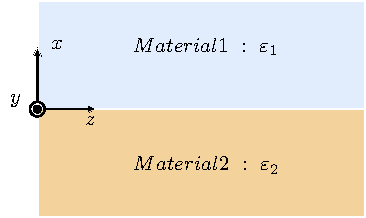
\includegraphics{figures/fig1}
  \caption{The SPPs exist on the interface of two different materials. Our considering surface is positioned in on the $yz$-plane.}
  \label{fig1}
\end{figure}


Here we are goin to find electromagnetic wave solutions ($\vb{E}(x,y,z,t),\vb{H}(x,y,z,t)$) that can be exist on the metal–dielectric interface. We represent the electric field of the SPP using $\vb{E}$ and the magnetic field with $\vb{H}$. In this case, we hoping to find solutions with following properties:
\begin{itemize}
  \item Wave solutions propagte through the surface (we assume they propagate to $z$-direction) \\
  \begin{equation} \nonumber
    \vb{E} \approx e^{-i\omega t + ik_z z} \quad
    \text{and} \quad
    \vb{H} \approx e^{-i\omega t + ik_z z}.
  \end{equation}
  \item Wave solutions decay through the both mediums (in the perpendicular direction to the surface) \\
  \begin{equation} \nonumber
    \vb{E} \rightarrow 0 \quad
    \text{and} \quad
    \vb{H} \rightarrow 0 \quad
    \text{as} \quad
    x \rightarrow \pm \infty.
  \end{equation}
\end{itemize}

In this analysis we consider a two material interface as mentioned in Fig.~(\ref{fig1}). These materials have the permitivity values  $\varepsilon_1,\varepsilon_2$ respectively for the upper one and the lower one. Without loss of generality, we can assume that $|\vb{E}|$ and $|\vb{H}|$ are independent on $y$. Now we can find the solutions for $\vb{E}$ and $\vb{H}$ by defining them as following form
\begin{equation}
  \vb{E} (x,y,z,t) = \bm{\mathcal{E}}(x) e^{-i\omega t + ik_z z}
  \quad \text{and} \quad
  \vb{H} (x,y,z,t) = \bm{\mathcal{H}}(x) e^{-i\omega t + ik_z z}.
\end{equation}
Furthermore, we restrict our study on to the TM-polarization mode as given in the Fig.~(\ref{fig1}). That means, we can represent the magnitudes of electric field and magnetic field as components of cartesian coordinate system
\begin{equation}
  \bm{\mathcal{E}} = (\mathcal{E}_x,\mathcal{E}_y,\mathcal{E}_z)^T
  \quad \text{,} \quad
  \bm{\mathcal{H}} = (\mathcal{H}_x,\mathcal{H}_y,\mathcal{H}_z)^T,
\end{equation}
with
\begin{equation}
  \mathcal{E}_y = 0 \quad,\quad \mathcal{H}_x = 0
  \quad,\quad \mathcal{H}_x = 0,
\end{equation}
and this leads to
\begin{equation}
  \bm{\mathcal{E}}(x) = \Big(\mathcal{E}_x(x),0,\mathcal{E}_z(x)\Big)^T
  \quad \text{,} \quad
  \bm{\mathcal{H}}(x) = \Big(0,\mathcal{H}_y(x),0\Big)^T.
\end{equation}
Next, to calculate known paramters, we can use Maxwell's equations
\begin{equation}
  \curl{\vb{H}} = \pdv{\vb{D}}{t} \quad \text{with} \quad
  \vb{D} = \varepsilon \varepsilon_0 \vb{E}
\end{equation}
\begin{equation}
  \curl{\vb{E}} = \pdv{\vb{B}}{t}\quad \text{with} \quad
  \vb{B} = \mu \mu_0 \vb{H},
\end{equation}
where $\varepsilon_0$ permitivity of vaccum. This will leas us to follwing set of equations
\begin{equation}
  -ik_z \mathcal{H}_y = -i \varepsilon \varepsilon_0 \mathcal{E}_x,
\end{equation}
\begin{equation}
  \pdv{\mathcal{H}_y}{x} = -i \varepsilon \varepsilon_0 \omega \mathcal{E}_z,
\end{equation}
\begin{equation}
  ik_z \mathcal{E}_x - \pdv{\mathcal{E}_z}{x} =
  i \mu \mu_0 \omega \mathcal{H}_y,
\end{equation}
and using these equation we can derive that
\begin{equation}
  \mathcal{E}_x = \frac{k_z }{\varepsilon \varepsilon_0} \mathcal{H}_y,
\end{equation}
\begin{equation}
  \mathcal{E}_z = \frac{i}{\varepsilon \varepsilon_0 \omega}
  \pdv{\mathcal{H}_y}{x},
\end{equation}
\begin{equation}
  \pdv[2]{\mathcal{H}_y}{x} -
  - \kappa^2 \mathcal{H}_y = 0 \quad
  \text{where} \quad
  \kappa = \pm\Big[k_z^2 - \mu\varepsilon \frac{\omega^2}{c^2}\Big].
\end{equation}
These quations known as the Helmholz equations and $c$ is the velocity of the light. We can identify the solution for above second order homogeneous differential equations as
\begin{equation}
  {\mathcal{H}_{y}}(x) = \mathcal{H} e^{-\kappa x}
\end{equation}
Here we only considered the positive solution for the $\kappa$ as we need only the decaying solution in outside of the interface and $\mathcal{H}$ is a unknown constant. Applying this solution into the two different mediums, we can find solutions for the electric and magneticfield in each medium as follows
\begin{itemize}
  \item Upper medium (Material1):\\
  \begin{equation}
    {\mathcal{H}_{1,y}}(x) = \mathcal{H}_1 e^{-\kappa_1 x} \quad,\quad
    {\mathcal{E}_{1,x}}(x) = \frac{k_z}{\varepsilon \varepsilon_0 \omega}\mathcal{H}_1 e^{-\kappa_1 x} \quad,\quad
    {\mathcal{E}_{1,z}}(x) = \frac{-i\kappa_1}{\varepsilon \varepsilon_0 \omega}\mathcal{H}_1 e^{-\kappa_1 x}.
    \end{equation}
    \item Lower medium (Material2):\\
    \begin{equation}
      {\mathcal{H}_{2,y}}(x) = \mathcal{H}_2 e^{\kappa_2 x} \quad,\quad
      {\mathcal{E}_{2,x}}(x) = \frac{k_z}{\varepsilon \varepsilon_0 \omega}\mathcal{H}_2 e^{\kappa_2 x} \quad,\quad
      {\mathcal{E}_{2,z}}(x) = \frac{i \kappa_2}{\varepsilon \varepsilon_0 \omega}\mathcal{H}_2 e^{\kappa_2 x}.
  \end{equation}
\end{itemize}
Here, $\mathcal{H}_1, \mathcal{H}_2$ are unknown constants which can be find by initial conditions and
\begin{equation}
  \kappa_1 = \sqrt{k_z^2 - \mu_1\varepsilon_1 \frac{\omega^2}{c^2}} \quad
  \text{,} \quad
  \kappa_2 = \sqrt{k_z^2 - \mu_2\varepsilon_2 \frac{\omega^2}{c^2}}.
\end{equation}

We can proceed further by considering the boundary condition of our system. Taking into account the boundary values we can identify the following identities
\begin{equation}
  {\mathcal{H}_{1,y}}(x =0) =  {\mathcal{H}_{2,y}}(x=0) ~\Longrightarrow~
  {\mathcal{H}_{1}} = {\mathcal{H}_{2}} = {\mathcal{H}},
\end{equation}
\begin{equation}
  {\mathcal{E}_{1,z}}(x =0) =  {\mathcal{E}_{2,z}}(x=0) ~\Longrightarrow~
  \frac{\kappa_1}{\varepsilon_1} = - \frac{\kappa_2}{\varepsilon_2}.
\end{equation}
Next, we assume these material are not magnatized materials ($\mu_1 =1,\mu_2 =1$), and this leads to
\begin{equation}
  \frac{\sqrt{k_z^2 - \varepsilon_1 {\omega^2}/{c^2}}}{\varepsilon_1} = - \frac{\sqrt{k_z^2 - \varepsilon_2 {\omega^2}/{c^2}}}{\varepsilon_2}
\end{equation}
Since the decaying parameters $\kappa_1,\kappa_2$ are defined as inverse of the penetration depth, we know these values should be get positive values. Therefore we can derive that one of the matrial's permitivity should be an negative value
\begin{equation}
  \varepsilon_1 \varepsilon_2 < 0.
\end{equation}
This implies that we can only find solutions for SSPs when one of the matrial should be a metal while onther one is a dielectric material. Therefore we can expext SPPs only on the metal-dielectric interfaces. Additionally, by solving above eqution we can identify the wave vector of the SPP's electric and magnetic field as
\begin{equation}
  k_z = \frac{\omega}{c} \sqrt{\frac{\varepsilon_1\varepsilon_2}{\varepsilon_1 + \varepsilon_2}}.
\end{equation}
























\end{document}
